\chapter{Proposta}\label{cap4}

\section{Usuários}


\section{Terminologias Existentes}

\subsection{Tesauros}

\subsection{Ontologias Existente}
Ontologias para a organização de \textit{audiobooks} são raras. Porém há uma grande similaridade entre ontologias para livros e para \textit{audiobooks}, uma vez que que tanto o livro quanto o áudio descrevem o mesmo conteudo. Mundando unicamente a forma que disponibilizam esse material. Dessa forma, a ontologia usada - nesse trabalho - para organizar ontologicamente um audiobook foi baseada uma ontologia desenvolvida por Naveen Kumar no intituto \textit{Ambedkar Institute of Advanced Communication Technologies}. 

A ontologia desenvolvida em Ambedkar deve cobrir uma ampla quantidade de informações e deve ter a capacidade para especificar as informções de formar a tornar mais eficas a pesquisa\cite{ontologybook}. A figura 2 mostra a abstração basica dos conceitos relacionados à livros e as relações semânticas. 

Existem basicamente quatro relações entre os conceitos: a relação de herança, relação de instância, relação parte-todo e relação sinoníma. A Relação de herança revela a relação de inclusão entre conceitos, ou seja, um subi-conceito é uma espécie de conceito pai, como por exemplo: ``Ruby of Rails'' é uma espécie de ``livro técnico'', em que ``livro técnico'' é um conceito pai, e ``Ruby of Rails'' é a sub-classe. A relação de instância é a relação da existência especifica de um conceito, como ``livro departamento de TI'' é uma instância de ``livro computador''. Relação parte-todo expressa um conceito que faz parte de um outro conceito, como ``manual de laboratório'' é parte do ``livro departamento de eletrônica''.

Não há informação semântica rica descrito explicitamente na ontologia. Podemos conhecer a partir da Figura 2 que o Java é um livro departamento CSE de livros de informática, e as pessoas podem chamá-lo pelo nome de ``OAK''. RDF (Resource Description Framework) e RDFS (RDF Schema) é um modelo de dados e mecanismo de apoio para a representação de meta-dados de esquemas \cite{rdf}, e é uma linguagem de representação de ontologias. RDF é um padrão baseado em XML para descrever recursos que existem na web, intranets e extranets. RDFS é usado para criar vocabulários que descrevem grupos de recursos RDF relacionados e as relações entre esses recursos. 


 \begin{figure}[ht]
	\centering
		\includegraphics[keepaspectratio=true,scale=0.5]{figuras/ontology.eps}
	\caption{Uma pequena parte da ontologia no dominio de livros.}
	\label{lanctocalivros}
\end{figure}





\section{Descrição do Ambiente Web}


\section{Cronograma}
A criação das atividades desse cronograma foram baseadas no plano de ensino da disciplina Tópicos especiais em Engenharia de Software. Este plano foi desenvolvido para o primeiro semestre letivo no ano de 2015.

 \begin{figure}[ht]
  \centering
    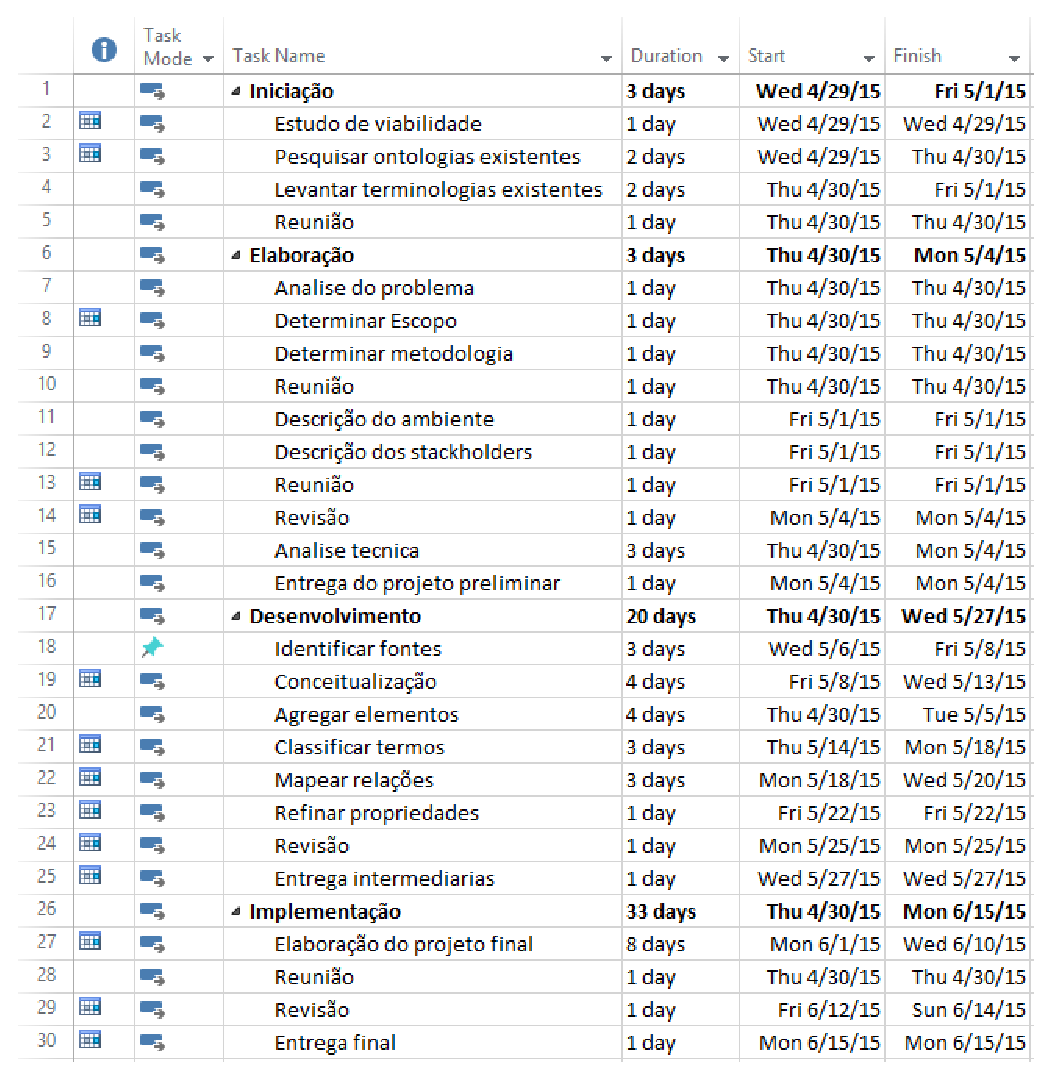
\includegraphics[keepaspectratio=true,scale=0.5]{figuras/cronograma.eps}
  \caption{Cronograma do projeto}
\end{figure}